\pagebreak
\section{Appendix}
\label{sec:appendix}
\newtheorem*{remark}{Remark}

\newcommand{\rp}{\right)}


% TODO: reorganize!

\subsection{Proof of Theorem \ref{thm:polytime}}

\begin{comment}
\begin{proof}
We assume without loss of generality that $S$ does not contain the all-zero string $\str_0$; if it does, since $\str_0$ can be meshed with any other string and so can always be released, we can solve the meshing problem for $S \setminus \str_0$ and then mesh each instance of $\str_0$ arbitrarily.

Rather than reason directly about the Min Clique Cover problem on some bounded-length meshing graph $G$, let us consider the equivalent problem of coloring $\bar{G}$, the complement of $G$.  $\bar{G}$ has an edge between  every pair of two nodes whose strings do not mesh.

$\bar{G}$'s node set $N$ can be partitioned into at most $2^b-1$ subsets $N_1, N_2, ... N_{2^b-1}$ such that $\forall i$, all nodes in $N_i$ represent the same string $\str_i$.  The induced subgraph of $N_i$ is a clique since all its nodes have a 1 in the same position and so cannot be pairwise meshed.  Further, all nodes in $N_i$ has the same neighbors since they all represent the same string.

Since $N_i$ is a clique, at most one node in $N_i$ may be colored with any color.  Fix some coloring on $\bar{G}$.  Swapping the colors of two nodes in $N_i$ does not change the validity of the coloring since these nodes have the same neighbor set.  We can therefore unambiguously represent a valid coloring of $\bar{G}$ merely by indicating in which cliques each color appears.

With $2^b$ cliques and a maximum of $n$ colors, there are at most $\lp n+1 \rp ^{2^{2^b}}$ such colorings on the graph.  This is polynomial in $n$ since $b$ is fixed, so we can simply check each coloring for validity (a coloring is valid iff no color appears in two cliques whose string representations mesh).  Finally, the algorithm returns a valid coloring with the lowest number of colors out of all valid colorings discovered.
\end{proof}
\end{comment}


We assume without loss of generality that $S$ does not contain the all-zero string $\str_0$; if it does, since $\str_0$ can be meshed with any other string and so can always be released, we can solve the meshing problem for $S \setminus \str_0$ and then mesh each instance of $\str_0$ arbitrarily.

Let $\bar G = (V, \bar E)$ be the complement of $G$.  Solving \textsc{MinCliqueCover} on $G(S)$ is equivalent to solving \textsc{Coloring} on $\bar G$.

\begin{lemma}
There are a polynomial number of colorings on $\bar G$.
\end{lemma}
\begin{proof}
Partition $V$ into $V_1, V_2, ... V_k$ such that $V_i = \{u \vert str(u) = s_i\}$.  Note that the induced subgraph of $\bar G$ on each $V_i$ is a clique, and further that $k \leq 2^b-1$.

Since $V_i$ is a clique, at most one node in $V_i$ may be colored with any color.  Fix some coloring on $\bar{G}$.  Swapping the colors of two nodes in $V_i$ does not change the validity of the coloring since these nodes have the same neighbor set.  We can therefore unambiguously represent a valid coloring of $\bar{G}$ merely by indicating in which cliques each color appears.

With $2^b$ cliques and a maximum of $|V| = n$ colors, there are at most $\lp n+1 \rp ^{2^{2^b}}$ such colorings on the graph.
\end{proof}

As a result of the lemma, we can check all colorings in polynomial time and return the minimum valid coloring.

\begin{remark}
This proof relies on the assumption that $b$, string length, is fixed.  This constraint limits meshing graphs to a strict subset of all possible graphs.  If $b = \bigo(n^2)$, any graph can be expressed as a meshing graph and so \textsc{MinCliqueCover} is NP-Hard in this case.
\end{remark}

\subsection{Experimental Confirmation of Maximum Matching/Min Clique Cover Convergence}

In Section~\ref{subsec:matching}, we argue that we can approximate the solution to \textsc{MinCliqueCover} on meshing graphs with high probability by instead solving \textsc{MaximumMatching}.

We experimentally verify this result by generating many random constant occupancy graphs and, for each graph, comparing the size of the maximum matching to the size of a greedy (non-optimal) solution for \textsc{MinCliqueCover}.  The results are summarized in Figure~\ref{plot:const}.

\begin{figure}[h]
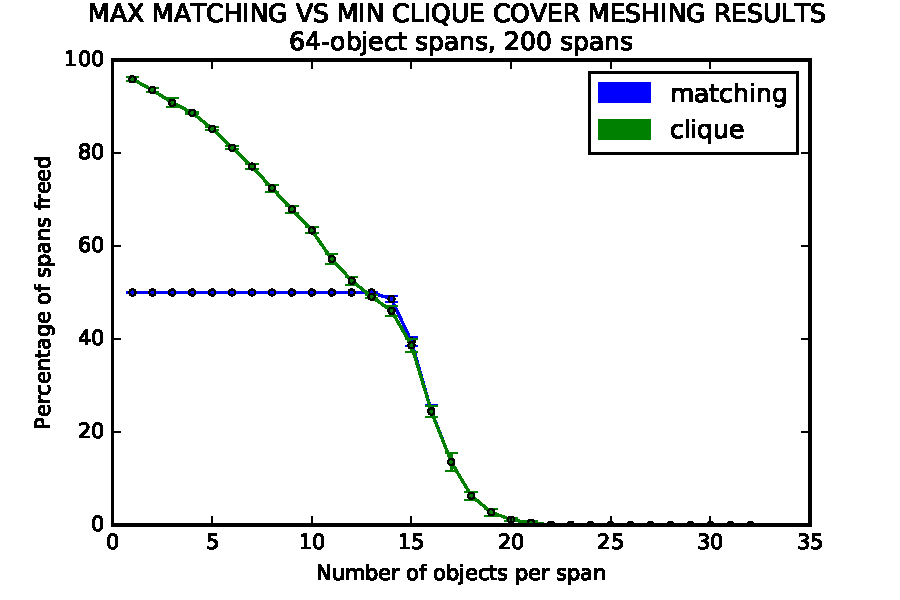
\includegraphics[scale = .5]{figures/const_match_comp.pdf}
\centering
\caption{\textbf{Min Clique Cover and Max Matching solutions converge.} The average size of Min Clique Cover and Max Matching for randomly generated constant occupancy meshing graphs, plotted against span occupancy.  Note that for sufficiently high-occupancy spans, Min Clique Cover and Max Matching are nearly equal.}
\label{plot:const}
\end{figure}



When we instead assume bits are 1 independently with probability p, we expect the graph to have many more triangles.  For $p = r/b = 10/32, n = 1000$, the expected number of triangles is roughly 36,000.  However, we can see experimentally that these graphs behave quite similarly in Figure~\ref{plot:indep}.


\begin{figure}[h]
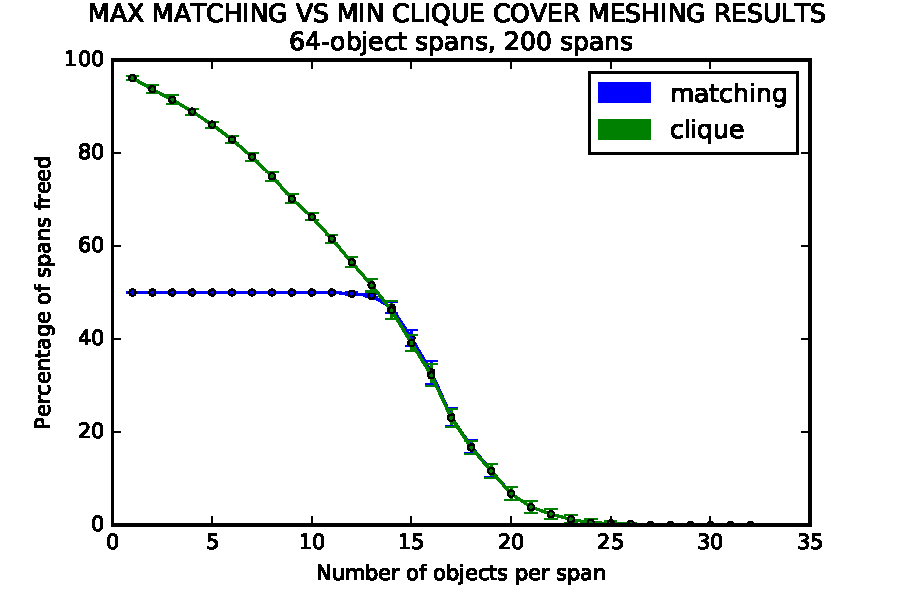
\includegraphics[scale = .5]{figures/ind_match_comp.pdf}
\centering
\caption{\textbf{Converge still holds for independent bits assumption.} The average size of Min Clique Cover and Max Matching for randomly generated constant occupancy meshing graphs, plotted against span occupancy.  Note that for sufficiently high-occupancy spans, Min Clique Cover and Max Matching are nearly equal.}
\label{plot:indep}
\end{figure}

While constant occupancy graphs are fairly regular, independent bit graphs may not be.  Since strings have different occupancies, nodes which correspond to strings with relatively low occupancy will tend to have significantly higher degree than other nodes in the graph.  Meanwhile, other nodes may have strings with high occupancy, and therefore only have a few edges (probably with low-occupancy nodes).  So while there are many triangles, when the graph is sparse enough, even meshing cliques of size 3 and 4 will likely "abandon" adjacent high-occupancy nodes, one of which could have been matched with the high degree node to yield the same number of releases.

So in this case we still expect finding the maximum matching to be good enough.

\iffalse
\subsection{Proof of Theorem 4.4}
\begin{proof}
Since spans all have identical occupancies, we expect the meshing graph to be nearly regular - the degree of each node is binomially distributed with mean $\lp n-1\rp q$.  When there are many objects per span, the degree distribution will be tightly concentrated around this mean.  For example, when $b = 128, n = 1000, q = .05$, the mean degree is 50 and less than 5\% of nodes have a degree greater than 60.

When we split the span set into half, and only consider pairs between the halves, we essentially remove half of the edges from the meshing graph.  To see this, observe that there are ${{n}\choose{2}} \approx n^2/2$ span pairs, and we fail to consider $2*{{n/2}\choose{2}} \approx n^2/4$ of them.  Note also that we fail to consider exactly $n/2 -1$ pairs for each span.  We therefore expect both the total number of edges in the meshing graph and the degree of each node to decrease by half.

How does the maximum matching of a graph change when you evenly sparsify the graph by half?  If the average degree is high enough, we expect this to not make much difference at all - each node in expectation still has many edges from which a matching can be built.

We can formalize this argument by first assuming that every node in the graph has degree at least $d$ and at most $\lp 1 + \epsilon \rp d$.  As we prove in Section~\ref{subsec:lowerbound}, the maximum matching of a graph $G = \lp V, E\rp$ is lower bounded by

$$W\lp G \rp = \sum_{\lp u,v \rp \in V} \min \lp \frac{1}{\degree \lp u \rp +1}, \frac{1}{\degree \lp v \rp +1} \rp$$

With our degree assumption we can further argue

\begin{align*}
W\lp G \rp \geq \sum_{\lp u,v \rp \in V} \frac{1}{\lp 1+\epsilon \rp d+1}
 \geq \frac{nd/2}{\lp 1+\epsilon \rp d+1}
\geq \frac{n}{2\lp 1+\epsilon \rp}
\end{align*}
and $W\leq n/2$.
%\lp G \rp &\leq \sum_{\lp u,v \rp \in V} \frac{1}{d+1} \leq \frac{n}{2}$
%\begin{align*}
%W\lp G \rp &\leq \sum_{\lp u,v \rp \in V} \frac{1}{d+1} \leq \frac{n}{2}
%\end{align*}

Note how these upper and lower bounds are independent of $d$ and $m$.  Thus, we decrease the maximum matching by at most a $1/\lp 1+\epsilon \rp$ factor by splitting the span set.
\end{proof}
\fi

\subsection{Proof of Theorem 4.5}
\begin{proof}
We begin by showing that the simpler quantity $W$ is a lower bound of the maximum matching $M$.
\[
W = \sum_{e\in E} \frac{1}{\max(\degree\lp u\rp, \degree\lp v\rp )+1}\ .
\]
%For each edge $e = (u,v) \in G$, define $\W$$(e)=min\lp \frac{1}{\degree\lp u\rp +1},\frac{1}{\degree\lp %v\rp +1}\rp$.  L
Let $U$ be an arbitrary set of $t$ nodes in $G$ where $t$ is odd.   Define $$W(U) = \sum_{u,v \in U} \frac{1}{\max(\degree\lp u\rp, \degree\lp v\rp )+1} \ . $$ As a corollary of Edmonds Matching Polytope Theorem, it can be shown that $W \leq M$ if  $W(U) \leq (|U|-1)/2$. We can argue this as follows:

\begin{align*}
W(U) &= \sum_{(u,v) \in U} \min \left(\frac{1}{\degree(u)+1},\frac{1}{\degree(v)+1}\right )\\
& \leq \sum_{(u,v) \in U}\frac{1}{2}\lp \frac{1}{\degree\lp u \rp +1}+\frac{1}{\degree\lp v\rp +1}\rp\\
&\leq \sum_{(u,v) \in U}\frac{1}{2}\lp \frac{1}{\degree_U\lp u\rp +1}+\frac{1}{\degree_U\lp v\rp +1}\rp\\
&= \frac{1}{2} \sum_{u \in U} \frac{\degree_U\lp u\rp }{\degree_U\lp u\rp +1} \leq  \frac{1}{2} \lp \frac{t-1}{t}\rp  t = \frac{t-1}{2}
\end{align*}
where $\degree_U(u)$ in the number of neighbors of $u$ in the set $U$.
The second line follows from the fact that the minimum of two quantities is bounded above by their average.  The third line follows from the fact that the degree of any node in a subgraph is bounded above by its degree in the original graph.  The fourth line follows from summing over nodes instead of edges, and then reasoning that in the worst case U is a clique and so $\degree_U(u) = t-1$ for all u $u$.

\iffalse
Recall that we prove in Section~\ref{subsec:lowerbound} that when
\[
w_e=\min\lp \frac{1}{\degree\lp u\rp+1 },\frac{1}{\degree\lp v\rp+1 }\rp
~~\mbox{ and }~~\W=\sum_{e\in E} w_e \ .\]
then $\W$ is a lower bound on the cardinality of the maximum matching M(G).
\fi


In some cases $W$ is too conservative; it assigns little weight to edges which it could safely have assigned much more.  For example, if $e$ is isolated (meaning its endpoints have degree 1), $W(e) = 1/2$.  However, it is always safe to assign weight 1 to $e$, since $M(G-e) = M(G)-1.$  If we modified our rule for $W$ so that for any edge $e= (u,v)$ s.t. $\deg(u)=\deg(v) = 1$ we assigned weight $ \min(1/\deg(u),1/\deg(v))$ instead of $ \min(1/\deg(u)+1,1/\deg(v)+1)$, we would always assign weight 1 to isolated edges.

In fact, a more general rule is true.  For any edge $e= (u,v)$, if either $\deg(u) or \deg(v) = 1$ then we may assign it weight $\min(1/\deg(u),1/\deg(v))$.

\iffalse
At this point it is natural to ask whether we can remove the $+1$s from the denominator for other edges.  We cannot of course do so for $\deg(u) = \deg(v) = k >1, k \in 2\mathbb{Z}$ since for a clique on k+1 nodes this rule would result in total weight $(k+1)/2$.\\

However, we can remove the $+1$ under certain circumstances. We show that if one of the endpoints has degree one then this is the case.
\fi

%prove several rules of this form.  For each rule we specify values of $\deg(u)$ and $\deg(v)$ for which the %$+1$ can be removed from the denominator of the edge weight.
%First we restate the claim that isolated edges may safely be assigned weight 1.
%\begin{lemma}
%Define $\W(G)$ as follows:\\
%For each $(u,v) \in G$,\\
%if $\deg(u) = \deg(v) = 1$, $\W(u,v) =  \min(\frac{1}{\deg(u)},\frac{1}{\deg(v)})$.\\
%else $\W(u,v) =  \min(\frac{1}{\deg(u)+1},\frac{1}{\deg(v)+1})$.
%Then $\W(G) \leq M(G)$.
%\end{lemma}
%\begin{proof}
%Already proven above.
%\end{proof}
%Next we will amend $\W$ to include the following rule: when one endpoint has degree 1 and the other has %degree k, assign weight $\frac{1}{k}$.

Define $\W$ as follows:
\[\W=\sum_{(u,v)\in E} \W(u,v) \]
where
\[
\W(u,v)=\frac{1}{\max(\degree\lp u\rp, \degree\lp v\rp )+I[\min(\degree(u),\degree(v))> 1]}\]

We now show that $\W \leq M$. We have proven that $W(U)\leq (t-1)/2$ on any odd-size subgraph $U$, $|U| = t$.  Define subsets $U_1$ and $U_2$ of $U$ such that $U_1 \cup U_2 = U$.  $U_1$ is the set of all nodes in $U$ of degree 1 and all nodes in $U$ adjacent to a node of degree 1, and $U_2$ is the set of all other nodes in $U$.  Let $G(U_2)$ denote the subgraph of $U$ induced by $U_2$, and let $|U_1| = x$ where x is even.  Then $W(G(U_2)) = \W(G(U_2)) \leq (t-x-1)/2$.  So to complete our proof we must show that all remaining edges (call them $E'$) have total weight $\leq x/2$.

Assume WLOG that there are no isolated edges in $G$ (if there are, we can group them with $G(U_2)$ and retain the $(t-x-1)/2$ bound).

\begin{align*}
\W(E') & \leq \frac{1}{2} \sum_{u,v \in E'} \lp \frac{1}{\deg(u)}+\frac{1}{\deg(v)}\rp\\
& = \mathlarger{\sum_k} \Big(\sum_{v \in U_1, \deg(v) = k} \frac{\delta}{k} + \frac{k-\delta}{2(k+1)}\Big)
\end{align*}
where $\delta$ denotes the number of degree 1 nodes adjacent to $v$.\\
Let $f(\delta) = \delta/k + (k-\delta)/(2(k+1))$.  We are interested in finding the maximum value $f(\delta)/(\delta+1)$ can take on; if it can never take a value greater than $1/2$ then $\W(E')$ cannot be greater than $x/2$.
$$\frac{\partial\frac{f(\delta)}{\delta+1}}{\partial \delta} = \frac{2-k}{2k(\delta+1)^2}$$
which is always negative for $k \geq 2$.  So, $f(\delta)/(\delta+1)$ is maximized at $\delta = 0$, so  $f(\delta)/(\delta+1) \leq k/(2(k+1)) < 1/2.$

There is one final detail we have not considered: $x$ might be odd.  In this case, $|U_2|$ is even and we can't appeal to Theorem 3 to say that $\W(G(U_2)) \leq (t-x-1)/2$.  However, we can simply remove one node $\node'$ from $U_2$; the resulting odd-size subgraph has weight at most $(t-x-2)/2$.  Since $\W$ is a valid fractional matching, the weight assigned to all edges adjacent to $\node'$ cannot exceed 1, so we can say that $\W(G(U_2)) \leq (t-x)/2$.  Now we must show that $\W(E') \leq (x-1)/2$.

We have shown that the edge weight per node in $U_1$ cannot exceed $1/2$.  $\W(E')$ is minimized when there is exactly 1 node of degree 1, with a degree k neighbor. In this case, the only edge in $E'$ will be assigned weight $k/(2(k+1))< 1/2$.  $\W(E') \leq 1/2 + (x-2)/2 = (x-1)/2$ and the theorem is proven.
\end{proof}

\iffalse
Finally, we further amend $\W$ to include the following rule:  when one endpoint has degree 2 and the other degree 3, assign weight $\frac{1}{3}$.

\begin{lemma}
Define $\W(G)$ as follows:\\
For each $(u,v) \in G$,\\
if $\deg(u) = 1$, or if $\deg(u) = 2$ and $\deg(v) = 3$, $\W(u,v) =  \min(\frac{1}{\deg(u)},\frac{1}{\deg(v)})$.\\
else $\W(u,v) =  \min(\frac{1}{\deg(u)+1},\frac{1}{\deg(v)+1})$.

Then $\W(G) \leq M(G)$.
\end{lemma}
\begin{proof}
Omitted for space.
\end{proof}
\fi
